\subsection{Kapitel 11}
Diese Kapitel fängt mit einer sehr interessanten Geschichte an. Der Turmbau von Babel. Über diese Geschichte tausende von Bilder. Es einer der Geschichten die man schon im Religionsunterricht in der Schule lernt. Der Bau eines riesigen Turms. Noch jetzt will der Mensch hoch hinaus. Es werden riesige Türme und Wolkenkratzer gebaut. Jeder angefressene Bergsteigen ist es ein Traum einmal auf dem höchsten Berg der Erde zu stehen. Und weil die Erde zu niedrig ist, werden jetzt Raketen und Raumschiffe ins Weltall geschickt. Aber auch im Sport auf der Arbeit in den Religionen heisst es oft, \frqq schneller, höher weiter \flqq{}.

Es ist im Menschen drin sich selber immer wieder zu übertreffen. Auch in der Bibel in vielen Geschichten manövrieren sich die Menschen in schlechte Situationen, nur weil sie sich selber, oder andere übertreffen wollen. Ich kenne es selber. Habe mit dem Rennrad die Strecken immer wieder verlängert. Gestartet mit 100km und am Schluss wollte ich die 1000km machen. Es war nur um mich selber zu bestätigen, dass ich das leisten kann. Quasi eine persönliche Befriedigung. Da diese Befriedigung nicht lange anhält, muss man immer wieder einen Schritt weiter gehen. Auch wenn nach so einem Ultrarennen alles schmerzte und ich während dem Rennen mir selber gesagt habe: \frqq nie wieder mache ich das!\flqq{} Habe ich nach einer Woche schon an der nächsten Herausforderung geplant.

In Babel hat Gott den Menschen da den Bau schnell eingestellt. 
\begin{figure}[ht]
    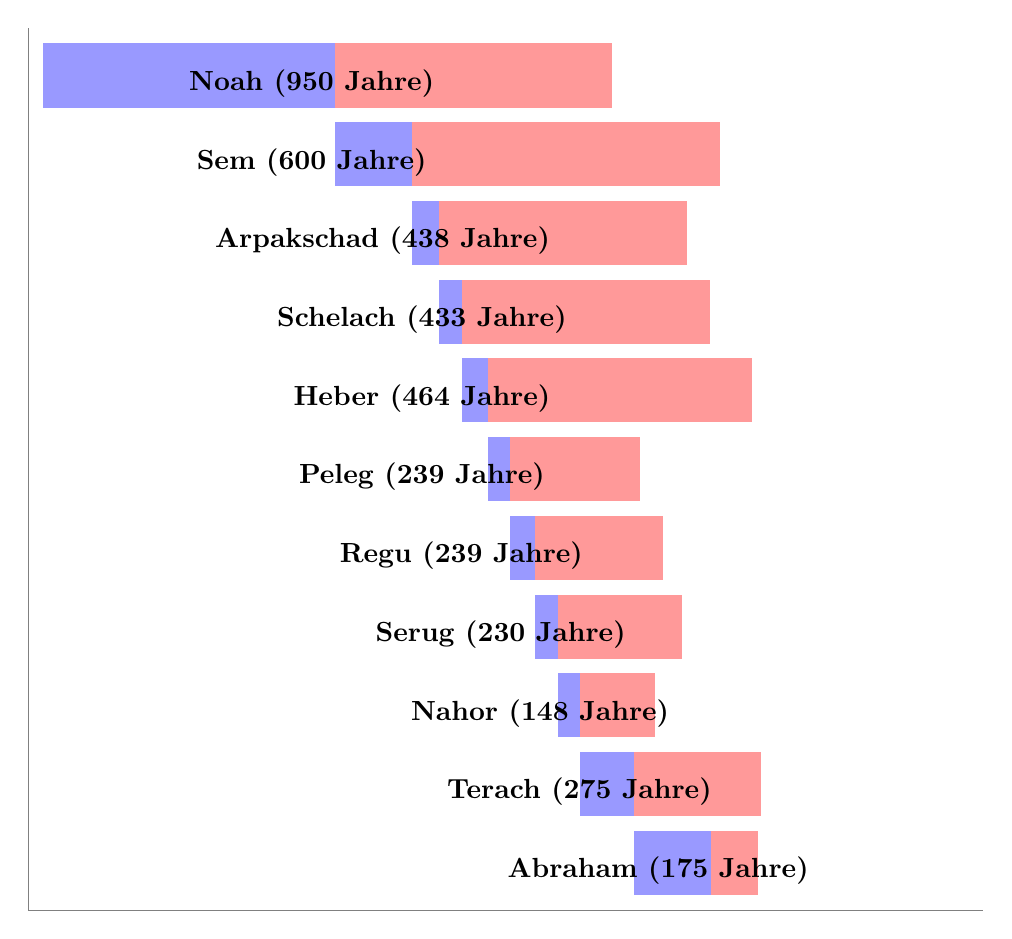
\begin{tikzpicture}
        \draw[gray] (0,0) -- (0mm, 112mm);
        %Noah 500-450 (0 - 93.6)
        \filldraw[blue!40] (2mm,110mm) rectangle(39mm,102mm);
        \filldraw[red!40] (39mm,110mm) rectangle(74.1mm,102mm) node at (36mm, 102mm) [right, above, black]{\textbf{Noah (950 Jahre)}};
        
        %Sem 100-500 (0 - 93.6)
        \filldraw[blue!40] (39mm, 100mm) rectangle(48.8mm,92mm);
        \filldraw[red!40] (48.8mm,100mm) rectangle(87.8mm,92mm) node at (36mm, 92mm) [right, above, black]{\textbf{Sem (600 Jahre)}};
        
         %Arpakschad 35-403 (15.6 - 62.4)
         \filldraw[blue!40] (48.8mm,90mm) rectangle(52.2mm,82mm);
        \filldraw[red!40] (52.2mm,90mm) rectangle(83.6mm,82mm) node at (45mm, 82mm) [left, above, black] {\textbf{Arpakschad (438 Jahre)}};
        
        %Schelach 30-403 (15.6 - 62.4)
        \filldraw[blue!40] (52.2mm,80mm) rectangle(55.1mm,72mm);
        \filldraw[red!40] (55.1mm,80mm) rectangle(86.5mm,72mm) node at (50mm, 72mm) [right, above, black] {\textbf{Schelach (433 Jahre)}};
        
        \filldraw[blue!40] (55.1mm,70mm) rectangle(58.4mm,62mm);
        \filldraw[red!40] (58.4mm,70mm) rectangle(91.9mm,62mm) node at (50mm, 62mm) [right, above, black] {\textbf{Heber (464 Jahre)}};
        
        \filldraw[blue!40] (58.4mm,60mm) rectangle(61.3mm,52mm);
        \filldraw[red!40] (61.3mm,60mm) rectangle(77.6mm,52mm) node at (50mm, 52mm) [right, above, black] {\textbf{Peleg (239 Jahre)}};
        
        \filldraw[blue!40] (61.3mm,50mm) rectangle(64.4mm,42mm);
        \filldraw[red!40] (64.4mm,50mm) rectangle(80.6mm,42mm) node at (55mm, 42mm) [right, above, black] {\textbf{Regu (239 Jahre)}};
        
        \filldraw[blue!40] (64.4mm,40mm) rectangle(67.4mm,32mm);
        \filldraw[red!40] (67.4mm,40mm) rectangle(83.0mm,32mm) node at (60mm, 32mm) [right, above, black] {\textbf{Serug (230 Jahre)}};
        
        \filldraw[blue!40] (67.4mm,30mm) rectangle(70.2mm,22mm);
        \filldraw[red!40] (70.2mm,30mm) rectangle(79.5mm,22mm) node at (65mm, 22mm) [right, above, black] {\textbf{Nahor (148 Jahre)}};
        
        \filldraw[blue!40] (70.2mm,20mm) rectangle(77mm,12mm);
        \filldraw[red!40] (77mm,20mm) rectangle(93.0mm,12mm) node at (70mm, 12mm) [right, above, black] {\textbf{Terach (275 Jahre)}};

        \filldraw[blue!40] (77mm,10mm) rectangle(86.8mm,2mm);
        \filldraw[red!40] (86.8mm,10mm) rectangle(92.6mm,2mm) node at (80mm, 2mm) [right, above, black] {\textbf{Abraham (175 Jahre)}};
        \draw[gray] (0,0) -- (\textwidth, 0mm);
    \end{tikzpicture}
    \caption{Lebensjahre von Noah bis Abraham}
    \label{balken_alter}
\end{figure}